\documentclass[a4paper]{article}

\usepackage[english]{babel}
\usepackage[utf8]{inputenc}
\usepackage{apacite}
\usepackage{graphicx}
\usepackage{tikz}
\usepackage{xcolor}
\usepackage[colorinlistoftodos]{todonotes}

\makeatletter
\def\BState{\State\hskip-\ALG@thistlm}
\makeatother

\title{Gameplay Design \\ Assignment 2 }

\author{
  Bowald, Johan\\
  \texttt{bowaldj@student.chalmers.se}
  \and
  Odbjer, Sebastian\\
  \texttt{sebastian.odbjer@gmail.com}
}

\date{\today}

\tikzset{
    vertex/.style = {
        circle,
        fill            = black,
        outer sep = 2pt,
        inner sep = 1pt,
    }
}

\begin{document}
\maketitle
\newpage

% Ricocheting Robots Game pettern analysis
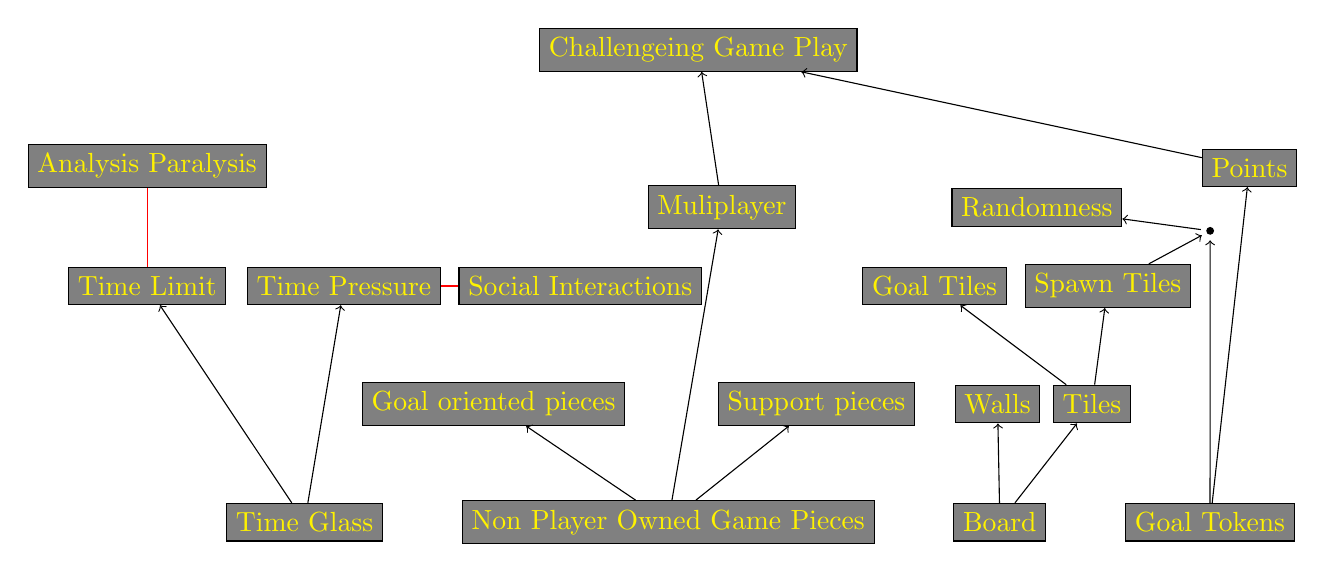
\begin{tikzpicture}
  \node[draw,fill=gray,text=yellow] (TimeGlass) at (-5,0) {Time Glass};
  \node[draw,fill=gray,text=yellow, right=of TimeGlass] (NPGP) {Non Player Owned Game Pieces};
  \node[draw,fill=gray,text=yellow, right=of NPGP] (Board) {Board};
  \node[draw,fill=gray,text=yellow, right=of Board] (GoalTokens) {Goal Tokens};

  \node[draw,fill=gray,text=yellow] at (-2.6,1.5) (GoalP) {Goal oriented pieces};  
  \node[draw,fill=gray,text=yellow] at (1.5,1.5) (SP) {Support pieces};  
  \node[draw,fill=gray,text=yellow] (Walls) at (3.8,1.5) {Walls};  
  \node[draw,fill=gray,text=yellow] (Tiles) at (5,1.5) {Tiles};  

  \node[draw,fill=gray,text=yellow] (TimeLimit) at (-7, 3) {Time Limit};  
  \node[draw,fill=gray,text=yellow] (TimeP) at (-4.5, 3) {Time Pressure};  
  \node[draw,fill=gray,text=yellow] (SI) at (-1.5, 3){Social Interactions};

  \node[draw,fill=gray,text=yellow] (MP) at (0.3, 4){Muliplayer};

  \node[draw,fill=gray,text=yellow] (SpawnT) at (5.2,3) {Spawn Tiles};  
  \node[draw,fill=gray,text=yellow] (GoalT)  at (3,3) {Goal Tiles};  

  \node[draw,fill=gray,text=yellow] (Randomness) at (4.3,4){Randomness};
  \node[draw,fill=gray,text=yellow] (Points) at (7,4.5) {Points};
  \node[draw,fill=gray,text=yellow, above=of TimeLimit] (AP) {Analysis Paralysis};
  \node[draw,fill=gray,text=yellow] (CGP) at (0,6) {Challengeing Game Play};

  \draw node[vertex] (JointGT) at (6.5,3.7) {};

  \draw[->,draw=black] (TimeGlass) to (TimeLimit);
  \draw[->,draw=black] (TimeGlass) to (TimeP);

  \draw[->,draw=black] (NPGP) to (GoalP);
  \draw[->,draw=black] (NPGP) to (SP);
  \draw[->,draw=black] (Board) to (Walls);
  \draw[->,draw=black] (Board) to (Tiles);  

  \draw[->,draw=black] (GoalTokens) to (JointGT);
  \draw[->,draw=black] (SpawnT) to (JointGT);
  \draw[->,draw=black] (GoalTokens) to (Points);
  \draw[->,draw=black] (JointGT) to (Randomness);

  \draw[->,draw=black] (Tiles) to (SpawnT);
  \draw[->,draw=black] (Tiles) to (GoalT);
  \draw[->,draw=black] (NPGP) to (MP);
  \draw[->,draw=black] (MP) to (CGP);
  \draw[->,draw=black] (Points) to (CGP);

  \draw[-,draw=red] (TimeLimit) to (AP);

  \draw[-,draw=red] (TimeP) to (SI);
  

\end{tikzpicture}
  


% \begin{tikzpicture}
%   % Dialectics
%   \node[draw,fill=gray,text=yellow] (DrawingStack) at (-1,0) {Drawing stack};
%   \node[draw,fill=gray,text=yellow] (Cards) at (2.3,0) {Cards};
%   \node[draw,fill=gray,text=yellow] (FixedDistributions) at (1,1.5) {Fixed Distributions};
  
%   \draw node[vertex] (Joint) at (1,0.5) {};
  
%   \draw[-,draw=black] (DrawingStack) to (Joint);
%   \draw[-,draw=black] (Cards) to (Joint);
%   \draw[->,draw=black] (Joint) to (FixedDistributions);
  
%   % Dice
%   \node[draw,fill=gray,text=yellow] (Dice) at (5,0) {Dice};

%   \node[draw,fill=gray!50,text=gray] (D4) at (3,-1) {D4};
%   \node[draw,fill=gray!50,text=gray] (D6) at (4,-1) {D6};
%   \node[draw,fill=gray!50,text=gray] (D8) at (5,-1) {D8};
%   \node[draw,fill=gray!50,text=gray] (D10) at (6,-1) {D10};
%   \node[draw,fill=gray!50,text=gray] (D12) at (7,-1) {D12};
%   \draw[->,draw=gray] (D4) to (Dice);
%   \draw[->,draw=gray] (D6) to (Dice);
%   \draw[->,draw=gray] (D8) to (Dice);
%   \draw[->,draw=gray] (D10) to (Dice);
%   \draw[->,draw=gray] (D12) to (Dice);
  
  
%   % Dice tier 2
%   \node[draw,fill=gray,text=yellow] (Randomness) at (4,2) {Randomness};
%   \node[draw,fill=gray,text=yellow] (Luck) at (6,2) {Luck};
  
%   \draw[->,draw=black] (Dice) to (Randomness);f
%   \draw[->,draw=black] (Dice) to (Luck);
    
%   % Dice tier 3
%   \node[draw,fill=gray,text=yellow] (LimitedForesight) at (2.2,3) {Limited Foresight};
%   \node[draw,fill=gray,text=yellow] (AnalysisParalysis) at (6,3) {Analysis Paralysis};
  
%   \draw[->,draw=black] (Randomness) to (LimitedForesight);
%   \draw[-,draw=red] (LimitedForesight) to (AnalysisParalysis);

%   \node[draw,fill=gray,text=yellow] (Surprises) at (1,4) {Surprises};
%   \draw[->,draw=black] (LimitedForesight) to (Surprises);
  
% \end{tikzpicture}

\newpage
\bibliographystyle{apacite}
\bibliography{bib}

\end{document} 

